\chapter{Conclusions}
\label{c:conclusions}

In this chapter, we describe our contributions, provide some discussion over our methodology and consider possible directions for future work.

\section{Contributions}

% We list below the contributions achieved with this dissertation.

Our most important contribution is a mechanisation using the \textit{Rocq Prover} and \textit{Autosubst} library of the following systems:
\begin{enumerate}
\item the multiary $\Lam$-calculus (system $\LamM$);
\item the canonical subsystem of $\LamM$;
\item the canonical $\Lam$-calculus (system $\LamV$).
\end{enumerate}

% There is no paper or computer formalisation of these systems with de~Bruijn indices that we know of.

Additionally, using these mechanised systems, we also obtained computer-verified proofs for results such as:
\begin{enumerate}
\item isomorphism between the canonical subsystem of $\LamM$ and system $\LamV$;
\item conservativeness of $\LamM$ over $\LamV$;
\item isomorphism between the simply typed $\Lam$-calculus and system $\LamV$;
\item subject reduction and confluence for systems $\LamM$ and $\LamV$.
\end{enumerate}

We can visualise some of these contributions in \cref{scripts_roadmap} by recalling our initial roadmap in \cref{roadmap}.
Each system and relationship is explicitly replaced by its corresponding script of formalisation.

% ---------------
\begin{figure}[h]
  \centering
  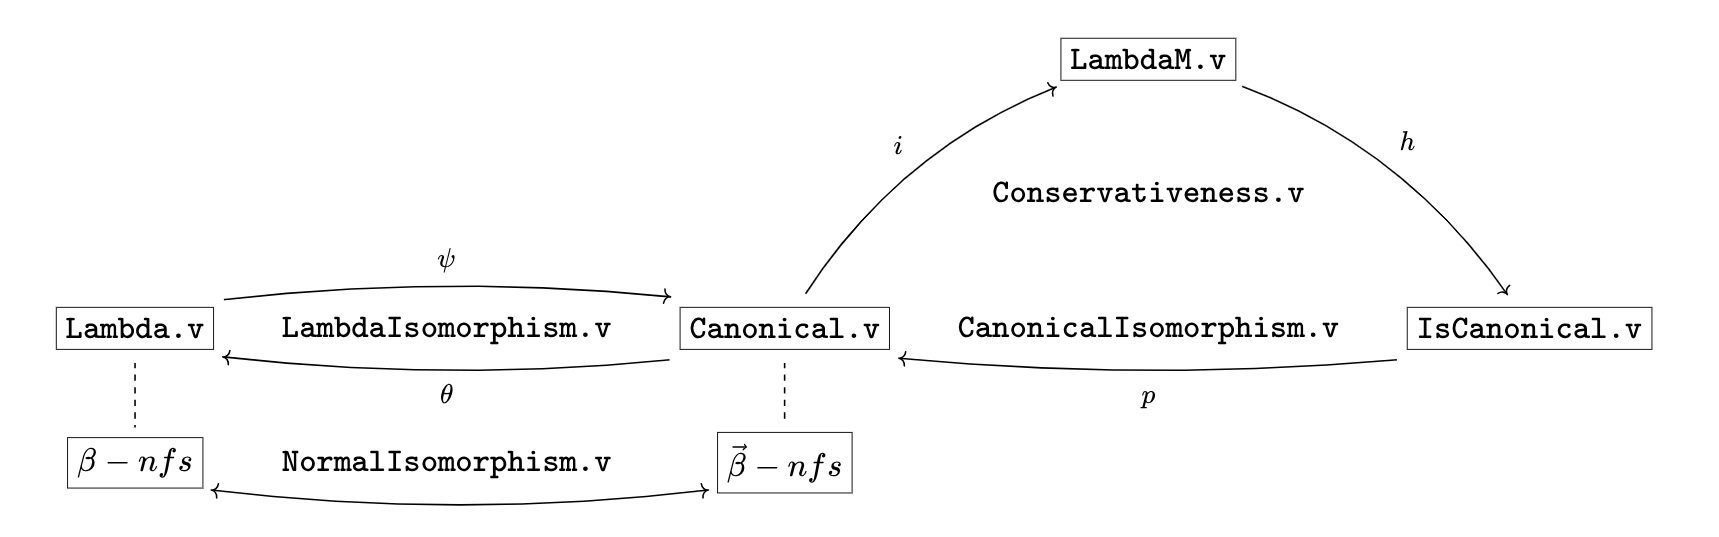
\includegraphics[width=1\textwidth]{pictures/scripts_roadmap}
  \caption{Roadmap of scrips in the \textit{Rocq Prover}} \label{scripts_roadmap}
\end{figure}
% ----------

We also see this document as a contribution, since we give a detailed exposition on how to use the \textit{Rocq Prover} to mechanise certain logical systems and mathematical results.
% along with some digressions over our formalisation choices.

A last contribution we emphasise is the in-depth study of the concept of subsystem.
By clarifying this often-loose definition, we separated two isomorphic representations of the canonical subsystem of $\LamM$.
For example, this clarification led us to simplify the statement and proof of the conservativeness theorem by using the self-contained system $\LamV$.

\section{Discussion and related work}

Before getting deeper into specific topics, we should mention two works that are in part related to ours.
First, a thesis \cite{AndrewAdams} that discusses many possibilities for mechanising a cut-free fragment of the sequent calculus and its relation with natural deduction, by experimenting with many proof assistants (including the former \textit{Coq}) and binding techniques (including de~Bruijn indices).
A second work \cite{Herbelin2017} that formalises metatheory of the first-order logical system \textit{LJT} using the \textit{Rocq Prover} is also interesting, because this system has a proofs-as-programs correspondence with the multiary system $\overline{\pmb \lambda}$ \cite{Herbelin1994}. 

Now, we provide some discussion over our mechanisation techniques, connecting them with related work.

\paragraph{De~Bruijn indices}
As already mentioned earlier, de~Bruijn indices (introduced in \cite{deBruijn}) is a technique to define a capture-avoiding substitution by working with expressions up to $\alpha$-equivalence.
In the original work of de~Bruijn, the use of parallel substitutions is already present, as a way to simplify the presentation of the substitution operation and at the same time generalising it.
This technique is often criticised for its unreadability and distance to the systems and results written in paper.

The literature is vast on other alternatives for representing syntax with binders \cite[Section~2.3]{POPLmark}.
Therefore, one can find a formalisation for the $\Lam$-calculus in these many flavours: nominal \cite{Vestergaard2001}, locally nameless \cite{McKinna1999} and HOAS \cite{Despeyroux1995}, to name a few.
We chose to use de~Bruijn syntax in the \textit{Rocq Prover} because there exists good support for this.
Adding to this, in our case, it was a way to avoid digressions over metatheory about $\alpha$-equivalence and capture-avoiding substitution that is not central to our work.

\paragraph{\textit{Autosubst} library}
The \textit{Autosubst} library \cite{AutosubstSchafer} was indeed a central choice along our work of formalisation using the \textit{Rocq Prover}.
It is an accessible tool for the mechanisation of metatheory of general syntax with binders.
It relies on the use of parallel substitutions and $\sigma$-calculus theory to simplify and automatise the metatheory around substitution operations.
Moreover, many of the operations provided for substitutions can work when using a general concept of typing systems with infinite contexts.

Other well-known libraries/code generators for mechanising syntax with binders in the \textit{Rocq Prover} are \textit{GMeta} \cite{GMeta} (a code generator for generic representations), \textit{Dblib} \cite{Dblib} (a library for representations using de~Bruijn indices) and \textit{LNGen} \cite{LNGen} (a code generator for locally nameless representations).
However, these libraries do not have support for expressions with many syntactical classes and we consider that they have a higher cost of entrance comparing to \textit{Autosubst}.

Another code generator that should be highlighted is \textit{Autosubst2} \cite{Autosubst2}.
Using the \textit{Autosubst} library seems an unusual choice, considering the existence of a code generator that appeared to fix many of its known problems, like not supporting many-sorted syntaxes.
Adding to this, many use cases prove its effectiveness in the mechanisation of metatheory \cite{Forster2019,Dudenhefner2024}.
We can argue for the use of the less sophisticated \textit{Autosubst} library in two ways.
First, we were able to achieve the desired support in the case of our systems thanks to the use of polymorphic lists.
Second, in the case of system $\LamV$ with a non conventional substitution operation, we would have nothing generated by \textit{Autosubst2}, as this system has an unexpected behaviour.
Using a library tool instead of a code generator allows us to use some working parts of the infrastructure and manually provide what is left.

\paragraph{Typing systems with infinite contexts}
Related with the choice of using the \textit{Autosubst} library, we recall the use of infinite contexts, or contexts as functions mapping natural numbers to simple types.
As already mentioned, this idea comes from the tutorial found in \cite{AutosubstManual}.
However, these are not the contexts that we work with in our paper proofs, thus, one would require a formal proof to admit this use.
We did not invest much on this and much like the case of de~Bruijn indices, we admit these facilities in order to invest our effort in the essential part of the metatheory.
Using this definition for contexts makes our statements simpler and allows using the \textit{Autosubst} operations and tactics already defined for substitutions because, in the proof assistant, contexts and substitutions over simple types have the same type (\lst$Gamma:var->type$).

\paragraph{Mechanising a subsystem}
In contrast to some decisions mentioned that facilitated our work of formalisation, the rigorous presentation of the canonical subsystem of $\LamM$ was one of our major efforts.
The task of mechanising a subsystem motivated us in this direction.
Recall that systems $\LamV$ and $\LamM$ correspond respectively to $\pmb{\lambda \mathcal{P}}$ and $\pmb{\lambda \mathcal{P} h}$.
In \cite[Chapter~3]{JCES2002}, system $\pmb{\lambda \mathcal{P}}$ is introduced as an isolated system that uses expressions from system $\pmb{\lambda \mathcal{P} h}$.

Our approach was to separate two different subsystems.
First, we defined what a subsystem of $\LamM$ was: a subset of expressions ($Can$ and $CanList$) closed under a notion of reduction and derivable sequent.
Afterwards, we wanted a direct, yet isomorphic, representation of this same subsystem ($\LamV$), with its appropriate notion of substitution.
A reduction over this ``self-contained'' canonical system is then defined and proved to be isomorphic to the induced notion of reduction for the canonical subsystem (the same is done for the typing systems).

In terms of the mechanisation, we found this useful.
It enabled us to work with a system with its own induction principles and many other dedicated definitions.
The downside to this technique was the need to prove an isomorphism.
An alternative could be the subset types provided in \textit{Rocq}, but this would rapidly become tiring because of the constant need to provide the proof object of a predicate defining the subset.

\section{Future work}

In this last section, we mention two directions that could be followed as a continuation of this dissertation.

% organization of work? modularisation and lemmas architecture - software engineering with mathematics
% We did not focus in results of confluency that could easily be added
% In this dissertation, we did not focus so much on results such as the confluency of reduction in our systems.
% We suspect that these could easily be added with the help of the \textit{Autosubst} library (one can found a case study of confluence of reduction in \cite[Section~2.2]{AutosubstSchafer}).

A first direction would be to extend the metatheory considered in our exercise of formalisation.
An initial approach could be to mechanise more metatheoretical results, such as strong normalisation for system $\LamM$.
Furthermore, we could extend our formalisation by enriching our systems with a more complex syntax (for example, system $\LamM$ is a subsystem of system $\pmb{\lambda J^m}$ from \cite{JCESLuis}).
A distinct and possible new way of work would involve generalising our typing systems beyond simple types - for instance, by incorporating polymorphism or dependent types.

A second and completely different direction would be to further explore the problems found in the mentioned libraries that aid the formalisation of syntax with binders.
From our experience using the \textit{Autosubst} library, we could suggest improvements in the automated tactics for deriving the substitution operation and substitution lemmas (motivated by our case with an unconventional substitution).
It would also be interesting to have a library containing many formalised systems and classical results (such as subject reduction, confluence, strong normalisation, etc...) using \textit{Autosubst} that could easily be used for in developments.

%%% Local Variables:
%%% mode: LaTeX
%%% TeX-master: "../dissertation"
%%% End:
